\documentclass[tikz]{standalone}
\usepackage{xcolor}
\usetikzlibrary{3d,calc}


\begin{document}
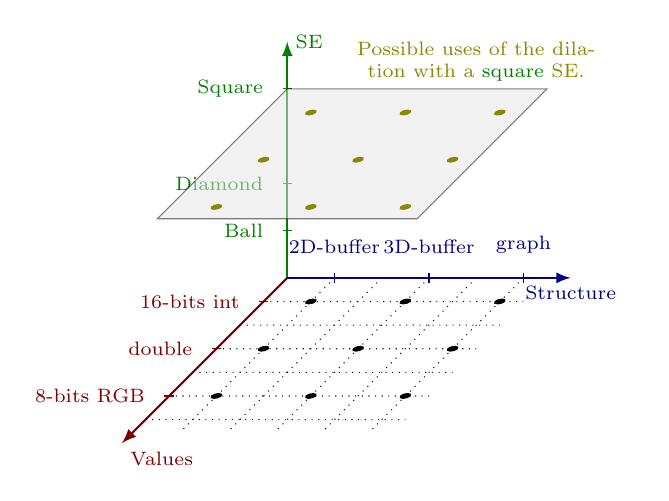
\begin{tikzpicture}[x  = {(1cm,0cm)},
                    y  = {(0cm,1cm)},
                    z  = {(-.5cm,-.5cm)},
                    scale=.6]

\scriptsize
\tikzset{
  SE/.style={left=.2cm, thick,
    append after command={+(-.1,0) -- +(.1,0)}
  },
  IM/.style={above=.2cm, thick,
    append after command={+(0,-.1) -- +(0,.1)}
  },
  VA/.style={left=0cm, left=.2cm, thick,
    append after command={+(-.1,0) -- +(.1,0)}
  },
  repere/.style={thick,-latex}
}

% Label 1
\draw[green!50!black,repere] (0,0,0) -- (0,5,0) node[right] {SE};
\draw[green!50!black] (0,1,0) node[SE] {Ball};
\draw[green!50!black] (0,2,0) node[SE] {Diamond};
\draw[green!50!black] (0,4,0) node[SE] {Square};

% Label 2
\draw[blue!50!black,repere] (0,0,0) -- (6,0,0) node[below] {Structure};
\draw[blue!50!black] (1,0,0) node[IM] {2D-buffer};
\draw[blue!50!black] (3,0,0) node[IM] {3D-buffer};
\draw[blue!50!black] (5,0,0) node[IM] {graph};

% Label 3
\draw[red!50!black,repere] (0,0,0) -- (0,0,7) node[below right] {Values};
\draw[red!50!black] (0,0,1) node[VA] {16-bits int};
\draw[red!50!black] (0,0,3) node[VA] {double};
\draw[red!50!black] (0,0,5) node[VA] {8-bits RGB};

% Lower plane
\begin{scope}[canvas is zx plane at y=0]
  \draw[black!90, dotted] (0,0) grid (6.5,5.5);
  \foreach \x in {1,3,5}
    \foreach \y in {1,3,5}
       \filldraw (\x,\y) circle (0.1);
\end{scope}

% Upper plane
\begin{scope}[canvas is zx plane at y=4]
  \filldraw[fill=gray!20,opacity=0.5] (0,0) rectangle (5.5,5.5);
  \node[above, olive, text width=4cm, align=center] at (0,4) {
    Possible uses of the dilation
    with a {\color{green!50!black} square} SE.
  };
  \foreach \x in {1,3,5}
    \foreach \y in {1,3,5}
       \filldraw[olive] (\x,\y) circle (0.1);
\end{scope}

\end{tikzpicture}
\end{document}


